%%%%%%%%%%%%%%%%%%%%%%%%%%%%%%%%%%%%%%%%%%%%%%%%%%%%%%%%%%%%%%%%%%%%
%% I, the copyright holder of this work, release this work into the
%% public domain. This applies worldwide. In some countries this may
%% not be legally possible; if so: I grant anyone the right to use
%% this work for any purpose, without any conditions, unless such
%% conditions are required by law.
%%%%%%%%%%%%%%%%%%%%%%%%%%%%%%%%%%%%%%%%%%%%%%%%%%%%%%%%%%%%%%%%%%%%

\documentclass[
  color, %% This option enables colorful typesetting. Replace with
         %% `monochrome`, if you are going to print the thesis on
         %% a monochromatic printer.
  table, %% Causes the coloring of tables. Replace with `notable`
         %% to restore plain tables.
  lof,   %% Prints the List of Figures. Replace with `nolof` to
         %% hide the List of Figures.
  lot,   %% Prints the List of Tables. Replace with `nolot` to
         %% hide the List of Tables.
  %% More options are listed in the class documentation at
  %% <http://mirrors.ctan.org/macros/latex/contrib/fithesis/fithesis/guide/mu/fi.pdf>.
]{fithesis3}
%% The following section sets up the locales used in the thesis.
\usepackage[resetfonts]{cmap} %% We need to load the T2A font encoding
\usepackage[T1,T2A]{fontenc}  %% to use the Cyrillic fonts with Russian texts.

\usepackage[
  main=english, %% By using `czech` or `slovak` as the main locale
                %% instead of `english`, you can typeset the thesis
                %% in either Czech or Slovak, respectively.
  german, russian, czech, slovak %% The additional keys allow
]{babel}        %% foreign texts to be typeset as follows:
%%
%%   \begin{otherlanguage}{german}  ... \end{otherlanguage}
%%   \begin{otherlanguage}{russian} ... \end{otherlanguage}
%%   \begin{otherlanguage}{czech}   ... \end{otherlanguage}
%%   \begin{otherlanguage}{slovak}  ... \end{otherlanguage}
%%
%% For non-Latin scripts, it may be necessary to load additional
%% fonts:
\usepackage{paratype}
\def\textrussian#1{{\usefont{T2A}{PTSerif-TLF}{m}{rm}#1}}
\usepackage{xcolor} 
\newcommand{\todo}[1]{\textcolor{red}{\textbf{#1}}}
\usepackage{listings}
%%
%% The following section sets up the metadata of the thesis.
\thesissetup{
    university    = mu,
    faculty       = fi,
    type          = bc,
    author        = Samuel Petrovic,
    gender        = m,
    advisor       = Adam Rambousek,
    title         = {The effects of age on file system performance},
    TeXtitle      = {The effects of age on file system performance},
    keywords      = {filesystem, xfs, IO operation, aging, fragmentation ...},
    TeXkeywords   = {filesystem, xfs, IO operation, aging, fragmentation ...},
}
\thesislong{abstract}{
    This is the abstract of my thesis, which can

    span multiple paragraphs.
}
\thesislong{thanks}{
    This is the acknowledgement for my thesis, which can

    span multiple paragraphs.
}
%% The following section sets up the bibliography.

\usepackage{csquotes}
\usepackage[              %% When typesetting the bibliography, the
  backend=bibtex,          %% `numeric` style will be used for the
  style=numeric,          %% entries and the `numeric-comp` style
  citestyle=numeric-comp, %% for the references to the entries. The
  sorting=none,           %% entries will be sorted in cite order.
  sortlocale=auto         %% For more unformation about the available
]{biblatex}               %% `style`s and `citestyles`, see:
%% <http://mirrors.ctan.org/macros/latex/contrib/biblatex/doc/biblatex.pdf>.
\addbibresource{citations.bib} %% The bibliograpic database within

                          %% the file `example.bib` will be used.
\usepackage{makeidx}      %% The `makeidx` package contains
\makeindex                %% helper commands for index typesetting.
%% These additional packages are used within the document:
\usepackage{paralist}
\usepackage{amsmath}
\usepackage{amsthm}
\usepackage{amsfonts}
\usepackage{url}
\usepackage{menukeys}
\usepackage{mwe}
\renewcommand{\lstlistingname}{Example}
\renewcommand{\lstlistlistingname}{List of \lstlistingname s}
\begin{document}
\chapter{Introduction}
File systems remain an important part of modern storage solutions.  Large, growing databases, multi-media and other storage based applications need to be supported by high-performing infrastructure layer of storing and retrieving information. Such infrastructure have to be provided by operating systems (OS) in form of file system.

Originally, file system was a simple tool developed to handle communication between OS and physical device, but today, it is a very complex piece of software with large set of tools and features to go with. Performance testing is an integral part of development cycle of most of produced software. Because of growing complexity of file systems, performance testing took of as and important part of file system evaluation.

The standard workflow of performance testing of file systems is to run benchmark (e.g. testing tool) on a clean instance of OS and on a clean instance of tested file system~\cite{fsbench-article:qhe}. Generally, this workflow present stable and meaningful results, yet, it only gives overall idea of file system behavior in early stage of its life cycle. 

File systems, as well as other complex software is subjected to progressive degradation, referred to as software aging~\cite{Cotroneo:2010:SAA:1913797.1914413}. Causes of file system aging are many, but mostly fragmentation of free space, unclustered blocks of data and unreleased memory. This degradation cause problems in performance and functionality over time. Understanding of performance changes of aged file system can help developers in implementing prevention . Such testing fundamentally consists of two steps. First is to bring fresh file system to an aged state and second is the actual performance test of the aged instance.

Foremost, this thesis describe implementation of flexible tests which represent the aforementioned steps. The first test is able to age fresh file system and store the result as an image for later use. The performance statistics collected in the process, as well as resulting layout can be used to evaluate ability of file system to respond to aging. Second test can evaluate resulting image even further by releasing some space and conducting performance test on resulting layout.

Furthermore, using developed tests to test different configurations of file systems and storage is demonstrated. The subject of research are differences between popular Linux file systems (XFS, Ext4) and storage technology (HDD, SSD) in context of aging. Because of nature of collected data, a processing tool was implemented to parse large amount of information into human readable reports. All the generated reports are part of this thesis in form of Appendix A.

The aging tests implemented in this thesis are established as part of testing cycle in Red Hat Kernel Performance team.

In the second chapter, the text present already conducted research of this topic. Third chapter introduce tools used in implementation of tests, while describing their relevant features.
\chapter{Previous research}





%%The standard workflow is tu run benchmark clean instance of operating system without other applications running, to avoid noise, and on clean instance of researched file system.

%%While this approach brings great results, with correct configuration of the benchmark, it only gives researchers a general idea about how does file system perform in early stage of it's usage. 

%%However, there is a growing demand from users as well as from file system developers to explore behavior and performance of a file system, that has been used for longer period of time.



%%This introduces problem in regard of devices with moving parts, such as widely used hard disk drive. When working with I/O operations on this type of device, the fragmentation cause larger seek times, which is a time for magnetic heads to reach desired location. This is a great example of how file system has to be flexible to solve such problems as well as of problems that emerge after running file system for a longer period of time.

%%The ideal approach of research pointed on effect on age of file system would be to put file system under defined conditions for a few years or months, gathering information in the process. However, this is apparently impractical or even impossible, because the demand for results has to be satisfied in matter of weeks to respond to new versions of file systems, which are developed and released quite often.

%%One of the earliest ideas about how to deal with this problem would be to capture a snapshot of a file system that had already been used for a prolonged time. This approach of testing on such a snapshot, however, would probably lead to optimising for a very specific instance of old version of given file system. 

%%If researchers want to predict behavior of a new version of file system after prolonged time of usage, they should be able to create a simulation, which would mimic the aging process, but in short period of time.
%%Aim of this thesis is to create 
%%This can be technically implemented, because the idea is to run the simulation continuously under very heavy workload without using operations which does not alter file systems layout, therefore researchers should be able to compress the time of creating such an aged file system in a short period of time.

%%Unfortunately the demand from users and developers has yet not been met by standard studies. There has been few studies executed in last millenium, that shed some light on this topic, but overall, modern research is in hands of regular users, remaining in amateur sphere, lacking professional equipment to execute such research properly.

%%The aim of this thesis is to create standard, configurable workflow of creating and storing aged file system as well as a workflow to mesure its performance. Workflow for file system aging will use open source tool fs-drift to simulate aging process and then creates and stores file system image using system tools. Workflow for performance testing will then use created images to perform various tests.

%%These workflows will then be used to test XFS and EXT4 file systems on different storage media to show their strenghts and weaknesses in respect to long time runnign, while showing importance of this kind of testing.

%%The conclusion of research will show how does aging affect hard drive disks compared to solid state disks, what effect has aging on file system performance and what are the performance differences between XFS and EXT4 after long time usage.

%%The workflows created for this thesis will be included in Red Hat File system performance testing campaigns.


\chapter{File systems}
In this chapter, I present basic information about file systems and describe main features of chosen file system in regard of fragmentation and scalability, which are important topics when discussing file system aging.

File system is a set of tools, methods, logic and structure to control how to store and retreive data on and from device.

The system stores files either continuously or scattered across device. The basic accessed data unit is called a block, which capacity can be set to various sizes. Blocks are labeled as either free or used.

Files which are non-continous are stored in form of extents, which is one or more blocks associated with the file, but stored elsewhere.  

Information about how many blocks does a file occupy, as well as other information like date of creation, date of last access or access permissions is known as metadata, e.g. data about stored data. This information is stored separately from the content of files. On modern file systems, metadata are stored in objects called index nodes (e.g. inodes). Each file a file system manages is associated with an inode and every inode has its number in an inode table. On top of that the file system stores metadata about itself (unrelated to any specific file), such as information about bad sectors, free space or block availability in a structure called superblock.

In this thesis, targeted file systems are two most popular Linux file systems, XFS and Ext4~\cite{Lu:2014:SLF:2578042.2560012}, which are also main Red Hat supported file systems. These file systems belong to the group of file systems called journaling file systems.

Journaling file system keeps a structure called journal, which is a buffer of changes not yet commited to the file system. After system failure, these planned changes can be easily read from the journal, thus making the file system easily fully operational, and in correct and consistent state again.

\section{XFS}
XFS~\cite{xfs:page} is a 64-bit journaling file system known for its high scalability (up to 9 exabytes) and great performance. Such performance is reached by architecture based on allocation groups.

Allocation groups are euqally sized linear regions within file system. Each allocation group manages its own inodes and free space, therefore increasing parallelism. Architecture of this design enables for significant scalability of bandwidth, threads, and size of file system, as well as files, simply because multiple processes and threads can access the file system simultaneously.

XFS allocates space as extents stored in pairs of B+ trees, each pair for each allocation group (improving performance especially when handling large files). One of the B+ trees is indexed by the length of the free extents, while the other is indexed by the starting block of the free extents. This dual indexing scheme allows efficient location of free extents for I/O operations.

Prevention of file system fragmentation consist mainly of a features called delayed allocation and online defragmentation.

Delayed allocation, also called allocate-on-flush is a feature that, when a file is written to the buffer cache, substracts space from the free-space counter, but won't allocate the free-space bitmap. The data is held in memory until it have to be stored because of system call. This approach improves the chance, that the file will be written in a contiguous group of blocks, avoiding fragmentation and reducing CPU usage as well.

\section{Ext4}
Ext4, also called fourth extended filesystem is a 48-bit journaling file system developed as successor of Ext3 for Linux kernel, improving reliability and performance features. Ext4 is scalable up to 1 exbibyte (approx. 1.15 exabyte). Traditional Ext2 and Ext3 block mapping scheme was replaced by extent based approach similar to XFS, which positively affects performance.

Similarly to XFS, Ext4 use delayed allocation to increase performance and reduce fragmentation. For cases of fragmentation that still occur, Ext4 provide support for online defragmentation and e4defrag tool to defragment either single file, or whole file system.

\chapter{Used tools}
In this chapter, I presnet tools which were used to implement automated tests for creating and storing aged file systems and measuring their performance. I will describe the main features and means of their usage. All the presented tools are open source projects.

\section{Beaker}
Beaker is a project aimed at automating testing workflow. The software can reserve machine from a pool of labs, install OS and packages, configure environment and perform tasks. The whole process is guided by sequence of instructions in an XML format. Further, I will show few examples of beaker usage.

\lstset{language=XML, 
numbers=left, 
frame=single, 
commentstyle=\color{dkgreen}, 
basicstyle={\scriptsize\ttfamily}, 
keywordstyle=\color{blue}, 
%identifierstyle=\color{blue}, 
%stringstyle=\color{mauve},
captionpos=t,
showstringspaces=false,
breaklines=true,
breakatwhitespace=false,
tabsize=3,
caption={sdad},
}


\begin{lstlisting}[language=xml, caption={Specifying OS to be installed}][frame=single]
<distroRequires>
  <and>
    <distro_family op="=" value="RedHatEnterpriseLinux7"/>
    <distro_variant op="=" value="Server"/>
    <distro_name op="=" value="RHEL-7.2"/>
    <distro_arch op="=" value="x86_64"/>
  </and>
</distroRequires>
\end{lstlisting}

\begin{lstlisting}[language=xml, caption={Configuring environment using kickstart}][frame=single]
<kickstart>
  <![CDATA[
    install
    lang en_US.UTF-8
    skipx
    keyboard us
    rootpw redhat
    firewall --disabled
    authconfig --enableshadow --enablemd5
    selinux --enforcing
    timezone --utc Europe/Prague

    bootloader --location=mbr --driveorder=sda
    zerombr
    clearpart --all --initlabel --drives=sda
    part /boot --fstype=ext2 --size=200 --asprimary --label=BOOT --ondisk=sda
    part /mnt/tests --fstype=ext4 --size=40960 --asprimary --label=MNT --ondisk=sda
    part / --fstype=ext4 --size=1 --grow --asprimary --label=ROOT  --ondisk=sda
    reboot
    %packages --excludedocs --ignoremissing --nobase
    @core
    wget
    python
    dhcpv6-client
    dhclient
    yum
]]>
</kickstart>
\end{lstlisting}




\section{FIO}
Flexible Input/Output tool is a IO workload generator written by Jens Axboe. It is a tool well known for it's flexibility as well as large group of users and contributors. The flexibility is integral for conductuing less artifical and more natural performance tests. However, approaching more natural test behavior, stability of results drop, so ideal equilibrium between these two parameters has to be found.

FIO accept

%%priklad logu

 

\section{Fs-drift}
fs-drift is a very flexible aging test, that can be used to simulate lots of different workloads. The test is based on random file access and randomly generated mix of requests. These requests can be writes, reads, creates, appends, truncates or deletes.

At the beginning of run time, the top directory is empty, and therefore \textit{create} requests success the most, other requests, such as \textit{read} or \textit{delete}, will fail because not many files has yet been created. Over time, as the file system grows, \textit{create} requests began to fail and other requests will more likely succeede. File system will eventually reach a state of equilibrium, when requests are equaly likely to execute. From this point, the file system would not grow anymore, and the test runs unless one of the \textit{STOP} conditions are met (specified with parameters).

The file to perform a request on is randomly chosen from the list of indexes. If the type of random distribution is set to \textit{uniform}, all indexes have the same probability to be chosen, see \ref{fig:rand1}. However, if the type of random distribution is set to \textit{gaussian}, the probability will behave according to normal distribution with the center at index 0 and width controled by parameter \textit{gaussian-stddev}. This is usefull for performing cache-tiering tests. Please note, that file index is computed as modulo maximal number of files, therefore instead of accessing negative index values, the test access indexes from the other side of spectrum, see Figure \ref{fig:rand2}

Furthermore, fs-drift offers one more option to influence random distribution. After setting parameter \textit{mean-velocity}, fs-drift will choose files by means of moving random distribution. The principle relies on a simulated time, which runs inside the test. For every tick of the simulated time, the center of bell curve will move on the file index array by the value specified using \textit{mean-velocity} parameter. By enabling this feature, the process of testing moves closer to reality by simulating more natural patterns of file system access (the user won't access file system randomly, but rather works with some set of data at a time). On figure Figure \ref{fig:rand3}, you can see bell curve moving by 5 units two times.

\begin{figure}[!htb]
    \centering
    \begin{minipage}{\textwidth}
        \centering
        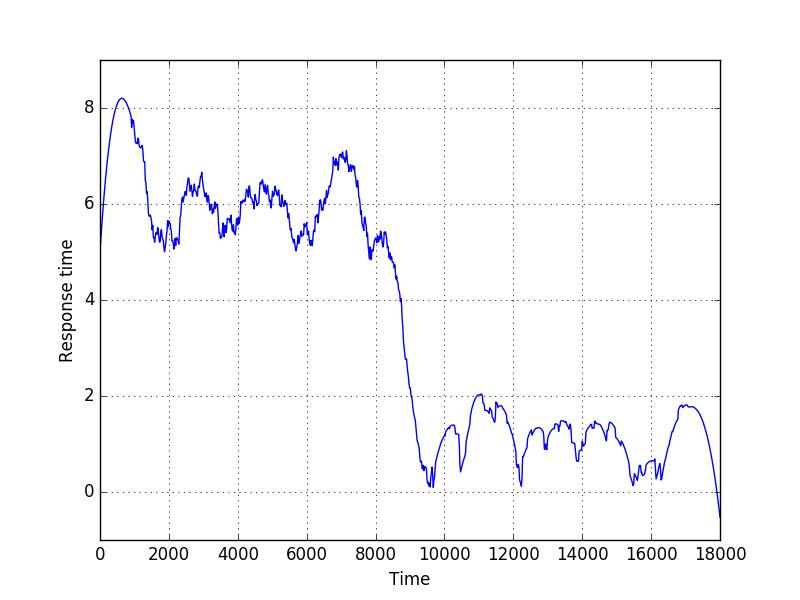
\includegraphics[width=0.7\textwidth]{../scripts/fig1.png}
        \caption{Uniform distribution of file access}
\label{fig:rand1}
    \end{minipage}\hfill
    \begin{minipage}{\textwidth}
        \centering
        \includegraphics[width=0.7\textwidth]{../scripts/fig2.png}
        \caption{Normal distribution of file access}

\label{fig:rand2}
    \end{minipage}

\end{figure}
\begin{figure}
    \begin{minipage}{\textwidth}
        \centering
        \includegraphics[width=0.7\textwidth]{../scripts/fig3.png}
        \caption{Moving random distribution}
\label{fig:rand3}
    \end{minipage}
\end{figure}

\section{Storage generator}

\chapter{Creating aged file system}

\section{File system images}
To achieve consistency of results and to shorten testing time, file system images are used. Once the image is created, it can be stored for later use and replayed back on device. To save space, only metadata of created file system are used, since content of created files is random and therefore irrelevant. Replayed metadata point at various blocks on device, recreating fragmentation while seldom taking significantly less space. These images can be created by using tools developed to inspect file systems in case of emergency. For ext based file systems, there is e2image tool and for xfs, there is xfs\_metadump. Both tools create images as sparse files, so compression is needed.

E2image tool can save whole ext based file system or just its metadata and offers compresion of image as well. Created images can be further compressed by tools such bzip2 or tar.

\noindent Creating compressed image using e2image:
\begin{lstlisting}[language=bash]
  e2image -Q $DEVICE $NAME.qcow2
\end{lstlisting}

\noindent Such images can be later replayed back on a device. From that point, file system can be mounted and revised.

\noindent Replaying compressed image:
\begin{lstlisting}[language=bash]
  e2image -r $NAME.qcow2 $DEVICE
\end{lstlisting}

Xfs\_metadump saves XFS file system metadata to a file. Due to privacy reasons file names are obsfucated (can be disabled by -o parameter). As well as e2image tool, the image file is sparse, but xfs\_metadump doesn't offer a way to compress the output. However, output can be redirected to stdout from where it can be passed to a compression tool. Creating compressed image using xfs\_metadump:

\begin{lstlisting}[language=bash]
  xfs_metadump -o $DEVICE -|bzip2 > $NAME
\end{lstlisting}

Such images, when uncompressed can be replayed back on device by tool xfs\_mdrestore. File system can be then mouned and inspected as needed:

\begin{lstlisting}[language=bash]
  xfs_mdrestore $NAME $DEVICE
\end{lstlisting}

%\section{filesystem\_ager}
%This aging tool is a simple approach to write and remove many files of random size.

%The tool consist of three scripts and one common library called \textit{functions}. The scripts are named \textit{filesystem\_ager.py}, \textit{fio\_config\_generator.py} and \textit{random\_deletor.py}.

%The workflow consist of calling filesystem\_ager, with desired parameters. Script manages triggering fio\_config\_generator, calling fio tool on generated config and triggering random deletor. These three actions are repeated given number of times.
%Parameters of filesystem\_ager are: 
%\begin{compactenum}
%  \item Total desired size do be written in one cycle
%  \item Denominator of total desired size (Total desired size will be divided by this number)
%  \item Range of size of written files
%  \item Number of cycles
%\end{compactenum}

%Although FIO tool has some parameters to randomize the size of files which are written, the management of file sizes and randomisation, as well as naming of files is handled by fio\_config\_generator instead, to provide more control over those qualities.
%Parameters of this script are:
%\begin{compactenum}
%  \item Total deisred size to be written
%  \item Range of size of written files
%\end{compactenum}

%The script will generate global settings of a workload, then proceeds to generate jobs for every file that will be written. File size is always the name of that file, and these are gathered to a list, then list of generated files is returned and script ends. Including file size in its name, as well as indexation of files will help effectively search and delete files in the random deletion process, without need to search for files on the disk and examine them for size. Simplistic approach in fio config will hopefully result in compatibility and reliability in use with any fio version.

%After config file is generated, filesystem\_ager will run fio tool on generated config and therefore, files are written on the device.

%The removing of files is handled by random\_deletor script. Its parameters are:
%\begin{compactenum}
%  \item Total written size
%  \item Denominator of total size
%  \item Range of size of written files
%  \item Number of existent files
%\end{compactenum}

%If denominator equals zero, random\_deletor wont remove any files and will return empty list. Otherwise, desired range of deletion is estimated. Random\_deletor then proceeds to remove files while desired volume is not deleted. Files are randomly selected through choosing random integer from zero to number of existent files. This step may seem inefficient, but with large amounts of generated files, the time to perform succesfull selection will not change dramatically. Selected file name is then parsed for size information, and if it fits into desired volume to remove, it is deleted, through subprocess command. Names of removed files are gathered in a list and returned.

%Number of deleted files is substracted from number of existent files.
%filesystem\_ager then sums up deleted volume, log it as well as other information and triggers the cycle again.

%However, after few runs, I decided not to use this approach for actual aging, because the time needed to fill and appropriately age the filesystem simply took very long. Instead, I was looking for other, already created tools I could use.

\section{Implementation}
Workflow of image creating is contained in the package drift\_job. After extracting fs-drift, the main script starts python script, which handles the process of running fs-drift. Settings of fs-drift are passed as a parameter and are parsed inside the script. Before running the fs-drift, python daemon thread is created to log free space fragmentation periodically while fs-drift is running. After the aging process is done, overall fragmentation is computed.

After the aging process, the script use system tools to create and compress the image. Information about system is gathered as well and all the logs are archived and sent to data collecting server.
Parameters available for drift\_job:
\begin{compactenum}
  \item -s|--sync, flag to signalise wheather or not to send data to server (usefull for developing purposes)
  \item -m|--mountpoint
  \item -d|--device
  \item -r|--recipe, parameters to pass to fs-drift
  \item -t|--tag, string to distinguish different tests
  \end{compactenum}

\section{Fs-drift/aging settings}
As the creator states in README, to fill up a file system, maximum number of files and mean size of file should be defined such that the product is greater than the available space. So if the workload is supposed to fill 500GB of space, while having maximum file size of 1GB (therefore mean size is 500MB), maximum number of files should be much higher than 1000. Optimal approach is to define seemingly no upper limit to let the fs-drift fill the volume, therefore numbers as high as $10^8$.

Parameter -t specifies the top directory, which will be used in test, in this workflow it is set to \$MOUNTPOINT.

There is an option to specifiy user-defined file to use as a workload table, which is a desired percentual representation of operations in a workload. Since the goal of this workload is to create fragmented file system in a short time, read and rename operations are irrelevant. Therefore only create, append and delete have representation in this workload. The optimal results were reached when every operation had equal representation, e.g. 33\%

The fs-drift allows directories up to defined level to create. The directory in which a file is directly affect its chance to be selected for a chosen operation, so by using only one directory, the equilibrium happens too fast, long before the file system is filled completely. Therefore we allow up to three levels of directories to be created.

Duration of the test is set to 5 hours so the test is usable for testing campaign without oversaturating of the servers.

\chapter{Performance testing of aged file system}

\section{Test structure}
Performance testing of created images is done by a package recipe\_fio\_aging. Upon instalation of necessary tools (libs, fio), the package finds and downloads coresponding file system image according to obtained parameters. As shown, images are stored compressed, therefore decompression is needed after download. Once these steps are succesfully completed, the image is restored on the device by using presented tools (e2image, xfs\_mdrestore). If the image restoring completes succesfully, file system can be mounted and worked with exactly like it would be just after the aging process.

After image restoration, some amount of the files needs to be deleted to create space for the performance test to take place. The files to be removed are chosen randomly until desired amount of volume has been freed. By using this workflow, e.g. freeing some amount of space, we can simulate aged file system in various phases of aging by using just one image of a very fragmented file system.

When free space is reclaimed, FIO test will take place using parameters given to recipe\_fio\_aging. The overall space occupied by the test should not be larger than available space on the file system, otherwise the test will either fail completely or report incorrect results.

For statistical correctness, the FIO test can run several times in a row. After last iteration, the results are archived and sent to data-collecting server.

Parameters available for recipe\_fio\_aging:
\begin{compactenum}
  \item -s|--sync, flag to signalise wheather or not to send data to server (usefull for developing purposes)
  \item -n|--numjobs, number of test repetitions. For statistical stability
  \item -m|--mountpoint
  \item -d|--device
  \item -r|--recipe, parameters to pass to FIO test
  \item -t|--tag, string to distinguish different tests
  \end{compactenum}

\section{Benchmark settings}
To ensure stability of test results, I decided to use simple form of standard performance test.
%Volume is randomly removed using random\_delete\_volume.py script. This scriptt globs all files in the filesystem, retrieves information about used volume as well as it's overall size. Then proceeds to randomly choosing files to delete and stops when desired volume is freed. The approach of recursively globbing all files may be inefficient, but this way, we can be sure, that volume is deleted from whole device evenly.

%\section{Inspecting filesystem}

%To determine overall idea about an extent to which is the file system aged, scripts that generate histograms representing fragmentation of used space as well as fragmentation of free space. Both scripts use common linux tools and pyplot to generate the graphics. Both scripts can display linear or logarhytmic Y scale.

%Script extent\_distribution.py makes use of xfs\_io fiemap tool, which is a tool to display extent distribution of a given file and works correctly even for ext* filesystems.

%The script will first recursively crawls the whole filesystem from given top folder and makes a list of all files. Fiemap is then run over every file separately. 

%The only data, that are then parsed from the output, is how many non-contigous extents does the file have. These integers are aggregated to a single list, from which are then counted, and final histogram is made.

%Script free\_space\_fragmentation.py use the tool e2freefrag, which runs over a device, and outputs the histogram of free space fragmentation in texutal form. Script will store this output and then easily parse the histogram and aggregate the data into a graphic form.

\chapter{Testing environment}
\section{Storage}
HDD is a rotational disk, which requires specific approach from kernel, to ensure the lowest possible seek time. Seek time is a time for moving parts of the device to find next relevant block of data. This affect overall performance greatly, because with large fragmentation, seek time becomes quite high.

As for SSD, this type of device does not have any moving parts, which make perform really well. One of the problems, however, is limited lifecycle of memory cells. SSD manufacturers deal with this problem by adding controler with its own scheduler, which make sure, no parts of the device are used significantly more than other parts.

When aging the filesystems, I expect for those grown on HDD to perform significantly slower after aging process, and I expect SSD filesystems not to be affected at all, or maybe significantly less.

\subsection{HDD}
\subsection{SSD}

\section{Used machines}
The aging process took place on these Machines:
\begin{compactenum}
  \item Model: LENOVO System x3250 M6
  \item CPU: Intel(R) Xeon(R) CPU E3-1230 v5 @ 3.40GHz (4 cores), arch i386 x86\_64 
  \item Memory: 16384 MB
  \item Storage: 
  \begin{compactenum}
	\item EG0600FBVFP HP Proliant HardDrive
	\item Interface: Serial Attached SCSI
	\item Capacity: 600 GB
	\end{compactenum}
\end{compactenum}  


\begin{compactenum}
  \item Model: IBM x3650 M4
  \item CPU: Intel(R) Xeon(R) CPU E5-2620 v2 @ 2.10GHz 
  \item Memory: 65536 MB
  \item Storage:
  \begin{compactenum}
	\item 2xSSDSC2BB480G4i IBM Solid State Drive
	\item Interface: Serial ATA
	\item Capacity: 480 GB
	\end{compactenum}
\end{compactenum}


The system installed on machines is RHEL-7.2 with kernel 3.10.0-514.el7.x86\_64 

\chapter{Results}
The output of result generator is a htlm report summarising all information about system, links to raw data and charts of measured values.

\section{Performance of aged file system}
\section{Differences betweem XFS and EXT4}
\section{Differences accross different storage}
\chapter{Conclusion}
Here I will admit, that these results were not really surprising and ABSOLUTELY no breakthrough, however, as noone really research this branch of QE, the results are definitely a step further in this field.

\printbibliography
\end{document}

